\section{TunnelMgr}\label{sec:tunmgr}

\begin{figure}
\begin{center}
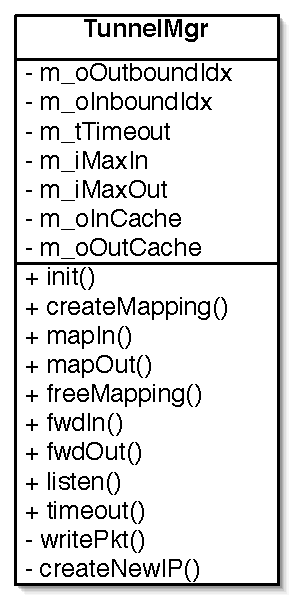
\includegraphics[width=0.4\textwidth]{figs/tunmgr}
\end{center}
\caption{}
\label{fig:tunmgr}
\end{figure}

This section describes the TunnelMgr component, which is described by Figure~\ref{fig:tunmgr}.  This component maintains a cache of
inbound and outbound connections.  These caches are instantiations of the LRU Cache class (described in Section~\ref{sec:lru}).  The
connections are placed in caches so that if connections are not properly cleaned up, the manager will not continue to maintain stale
connection mappings.

As outbound connections are made new mappings are created via the createMapping() method.  The results are then placed in the outbound
connection cache, and referenced by the outbound index (which is an STL map).  Similarly, inbound connections are managed by the inbound
analogs.  These structures are managed separately so that audit trails can be maintained about active inbound vs. outbound connections, and
so that logic can (potentially) be different when handling them.  Caches are filled with TunnelEntry objects that fully describe the
headers needed to encapsulate outbound packets, and the local IP address needed to forward inbound packets.

The main thread of the manager blocks on the listen() method which awaits incoming connections and outgoing packets (via a
select() call).  Outbound packets are passed the the fwdOut() method which creates the proper headers and encapsulates the packet.  
Inbound connections are handed to the fwdIn() method which tries to interpret the inbound headers and look them up in the inbound cache.

General convention for determining \textit{in/out} packets/methods: Generally, \textit{in} refers to packets read from the ListenFD, and meant to be pushed onto the TunFD. Correspondingly, \textit{out} refers to packets read from the TunFD and meant to be pushed onto the ListenFD.

\subsection{Methods}

{\bf Public Methods}
\begin{itemize}
\item init(): Initialize the internal state of the manager and clean up all data structures.
\item createMapping(): Create a new tunnel.  Map a new IP address to a set of TunnelEntry objects that specify the headers needed to
create the tunnel.  Place this mapping in the appropriate IP lookup cache and index.
\item mapIn(): Take an inbound packet and determine which internal IP address it belongs to and retrieve all state needed.
\item mapOut(): Take an outbound packet and determine what headers are needed to deliver it to the proper destination and retrieve all
state needed.
\item freeMapping(): Clean up state information from index and cache for a specific mapping (IP and tunnel headers).
\item fwdIn(): Take an inbound packet, lookup its mapping info, de-encapsulate, and format the packet for local delivery.
\item fwdOut(): Take an outbound packet, lookup its mapping info, encapsulate it for tunneling to a remote destination.
\item listen(): Await inbound connections on a network port.
\item timeout(): Check to see if any tunnels have been inactive for long enough that we can reclaim and free their state.
\end{itemize}

{\bf Private Methods}
\begin{itemize}
\item writePkt(): Given a set of headers or a new IP address encapsulate of de-encapsulate and return a routable packet.
\item createNewIP(): Perform the platform specific operations of allocating a new IP address in the local subnet.
\end{itemize}

\subsection{Member Variables}
\begin{itemize}
\item m\_oOutboundIdx: <placeholder>
\item m\_oInboundIdx: <placeholder>
\item m\_tTimeout: time\_t - This member is the amount of time an entry is allowed to be idle before it can be considered for removal.
\item m\_iMaxIn: int - This member is the maximum number of inbound mappings that may be kept.
\item m\_iMaxOut: int - This is the maximum number of outbound mappings that may be kept.
\item m\_oInCache: LruCache - This member maintains a lookup of TunnelEntry objects based on the IP address the inbound packet came from.
\item m\_oOutCache: LruCache - This member maintains a lookup of TunnelEntry objects based on the IP address the outbound packet came from.
\end{itemize}
